\chapter{Results}
From the earlier chapter I described the final form of the data output from the program.
Below is a sample from the Metropolis data file.
\begin{table}[h]
\centering
\begin{tabular}{ccc}
0    & 0             & 0.000277831 \\
0.05 & 0.00000183835 & 0.000301732 \\
0.1  & 0.00000759666 & 0.000289046 \\
...  & ...           & ...         \\
2.5  & 0.000177274   & 0.000889706 \\
2.55 & 0.000121696   & 0.000737807 \\
2.6  & 0.000113462   & 0.000829744
\end{tabular}
\end{table}

The Wang Landau output file looks like this
\begin{table}[h]
\centering
\begin{tabular}{cc}
-1.972222222   & 117.227  \\
-1.916666667   & 114.667  \\
-1.861111111   & 112.106  \\
...            & ...      \\
-0.1388888889  & -28.7273 \\
-0.08333333333 & -26.1667 \\
-0.02777777778 & -28.7273
\end{tabular}
\end{table}

Using this data we can start constructing the physical quantities and plotting them.

\section{Metropolis}
\subsection{Range of beta}
For the Metropolis data, the first step is to plot the data to ensure the program produced expected behaviour.
In this case expected behaviour for the Energy as a function of $\beta$ is that at low $\beta$, high T, the energy would be nearing it's maximum and that for high $\beta$, low T the energy would be close to its minimum and at there would need to be a transition between these two points.

\begin{figure}[H]
\centering
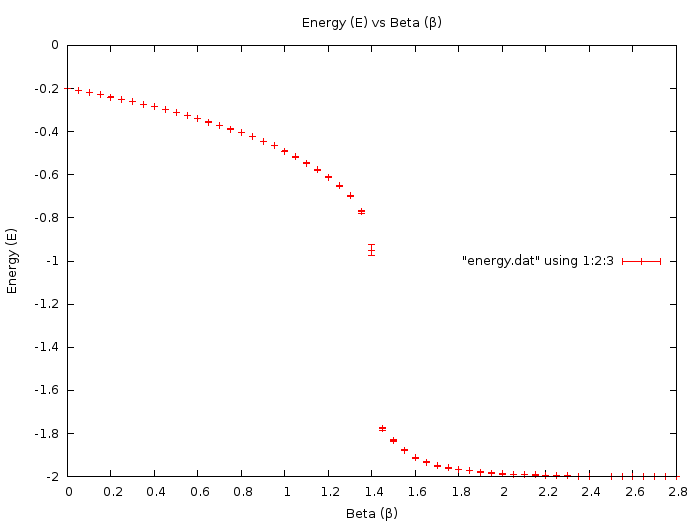
\includegraphics[width=0.75\textwidth]{4-Results/Q10EnergyBeta16x16RangeofBeta.png}
\caption{Graph showing Energy vs $\beta$}
\end{figure}

In the graph above, the expected behaviours are clearly visible. The data shows that the energy approaches it's maximum at low $\beta$ and it's minimum at high $\beta$. 
The above graph is set for $Q=10$ which has a phase transition at $\beta_c = \ln(1+\sqrt{Q}) \approx 1.426$ in the thermodynamic limit, while the graph clearly shows a transition it isn't at this $\beta_c$ but this is due to the finite size of the lattice used in this simulation.

For Magnetisation the expected behaviour is that for high $\beta$, low T, that magnetisation per unit volume would be equal to 1. At low $\beta$, high T, this property disappears and should approach a minimum. Again the expected behaviour is seen in the graph below. The phase transition occurs at around the same position as in the Energy case which is another quick check to make.

\begin{figure}[H]
\centering
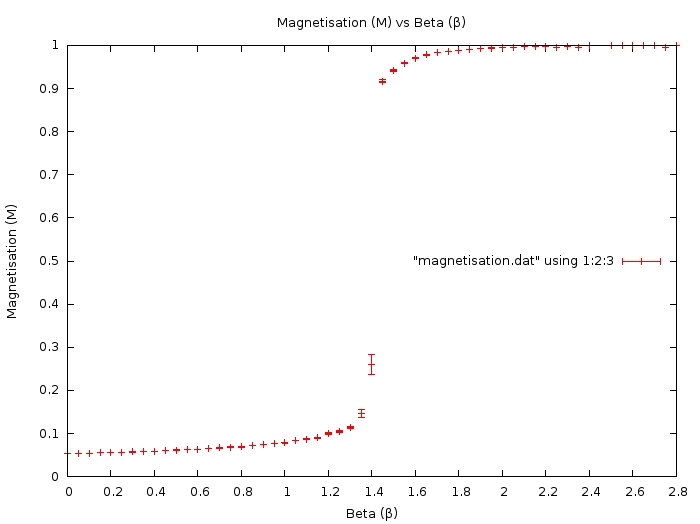
\includegraphics[width=0.75\textwidth]{4-Results/Q10MagnetisationBeta16x16RangeofBeta.png}
\caption{Graph showing Magnetisation vs $\beta$}
\end{figure}

For the other data files that are measured, which include the Specific Heat, C and the Magnetic Susceptibility,$(\chi)$ the behaviour should be 0 everywhere except at the phase transition as stated above, $\beta_c \approx 1.426$ in the thermodynamic limit.

\begin{figure}[H]
\centering
\begin{subfigure}[b]{0.45\textwidth}
    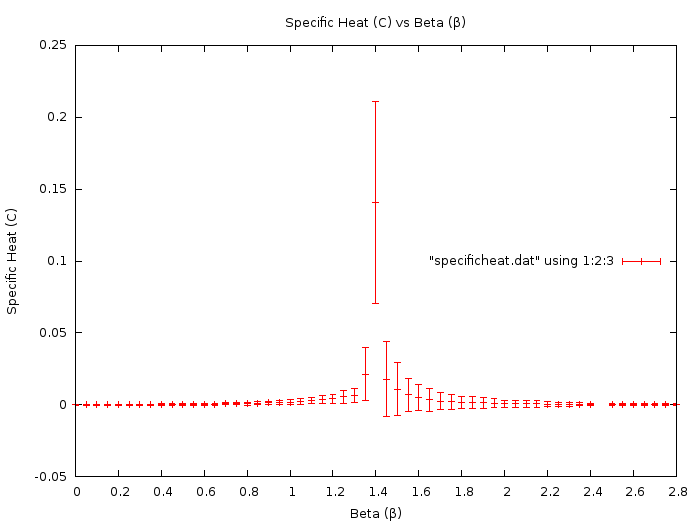
\includegraphics[width=\textwidth]{4-Results/Q10SpecificHeatBeta16x16RangeofBeta.png}
    \caption{Q10 Graph showing Specific Heat ($C$) vs $\beta$}
\end{subfigure}
\begin{subfigure}[b]{0.45\textwidth}
    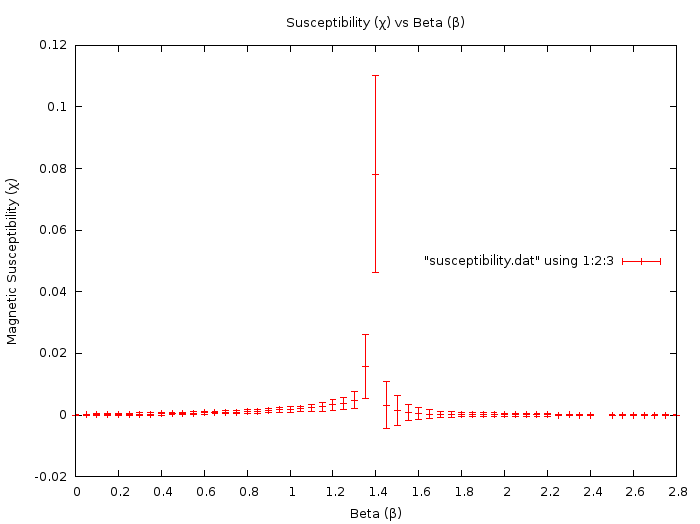
\includegraphics[width=\textwidth]{4-Results/Q10SusceptibilityBeta16x16RangeofBeta.png}
    \caption{Q10 Graph showing Magnetic Susceptibility ($\chi$) vs $\beta$}
\end{subfigure}
\end{figure}

The peaks in the two graphs above are obvious and fit with the expected results for the respective quantities.

While these quick checks are useful while debugging the code to ensure that the simulated behaviours are correct, on their own they don't provide enough information to verify the code is working correctly this will be dealt with in the next step.

\section{Wang Landau}

\subsection{Plotting the Output}
The first step of dealing with the Wang Landau output is, like the Metropolis, is to plot it.
This is to visually verify that the behaviour is as expected, in this case the iterative process for calculating $a_n$ leads to data that starts at an initial value $a_0$ and that will converge towards and oscillate around in a band of acceptable values.
\begin{figure}[H]
\centering
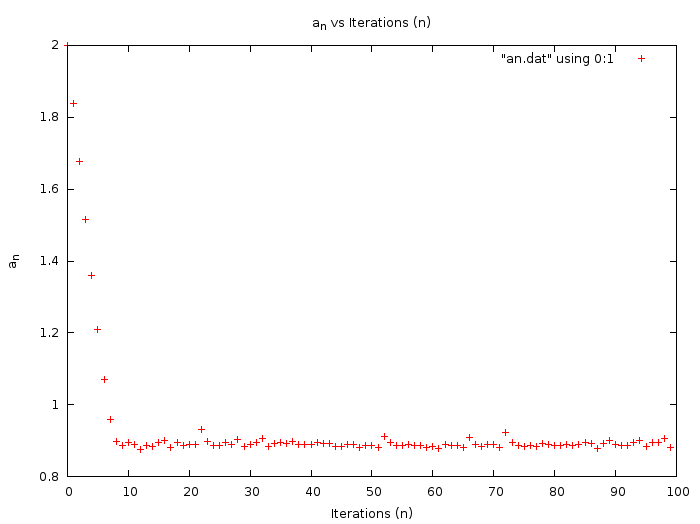
\includegraphics[width=0.75\textwidth]{4-Results/An16x16Convergence.png}
\caption{Graph showing the $a_n$ convergence vs n}
\end{figure}
It is clear that in the above graph the behaviour is as expected.
The value of $a_n$ converges extremely quickly towards it's target value and oscillates slightly around its value.

\subsection{Are the results compatible with the Metropolis?}
In an earlier section, I stated that the information provided by the metropolis wasn't enough information to verify the code was working correctly.
The Metropolis part of the program was a stepping stone to the implementation of the Wang Landau algorithm that was the primary portion of this project.
That being said, you can verify the results returned by the Wang Landau mode of this project by using the energy values returned by the Metropolis code at the $\beta_c$ at the thermodynamic limit. 
$a_n$ should be roughly equivalent to the $\beta$ required to keep the system at the target energy using this information and the value of $\beta_c$ I calculated the value of $a_n$ at the critical point using the energy value returned from the Metropolis data.
This leads to a data file looking similar to the one below.
\begin{table}[H]
\centering
\begin{tabular}{ccc}
8  & -1.74296 & 0.00591688 \\
10 & -1.72614 & 0.00648999 \\
12 & -1.71512 & 0.0058484  \\
14 & -1.69895 & 0.0067316  \\
...	& ...	& ...	\\
28 & -1.7049  & 0.00379986 \\
30 & -1.7069  & 0.00395975 \\
32 & -1.72059 & 0.00357536
\end{tabular}
\end{table}
The first column is the lattice size, the $2^{nd}$ column is the Energy at $\beta_c$ and the third column is the error in the $2^{nd}$ column.
Using this data I wrote several shell scripts that are designed to run the program in the Wang Landau mode using the target energy provided in the $2^{nd}$ column.
Taking the results from the Wang Landau mode of the program using the shell scripts described above to collect the values of $a_n$ for the various grid sizes you can plot them against the inverse volume.
At the thermodynamic limit, the inverse volume should be 0. If you fit the results with a linear function $y=ax+b$, it's intercept represents the value at the thermodynamic limit.
The intercepts for this particular test are shown in the table below.
\begin{table}[H]
\centering
\begin{tabular}{|c|c|c|c|}
\hline
Q  & Theoretical & Result   & Error    \\ \hline
2  & 0.881373587 & 0.865616 & 0.03173  \\ \hline
3  & 1.005052539 & 0.996294 & 0.01123  \\ \hline
4  & 1.098612289 & 1.11538  & 0.002026 \\ \hline
8  & 1.342454046 & 1.34759  & 0.008933 \\ \hline
10 & 1.426062439 & 1.43679  & 0.0152   \\ \hline
\end{tabular}
\end{table}

A plot of the data as it appeared is now provided below.

\begin{figure}[H]
\centering
\begin{subfigure}[b]{0.45\textwidth}
    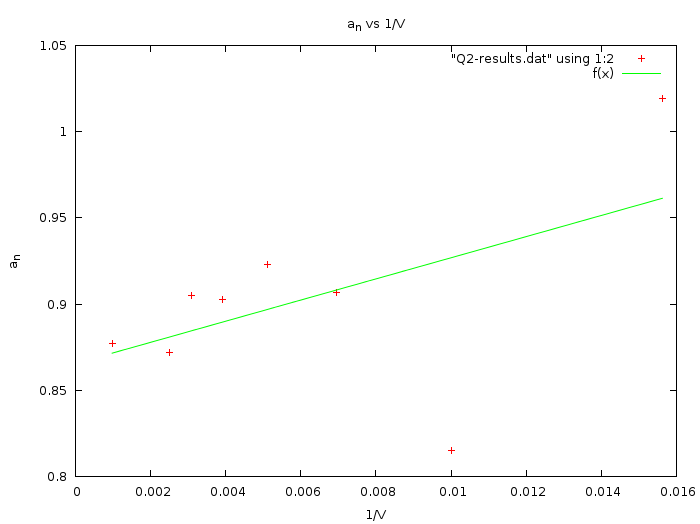
\includegraphics[width=\textwidth]{4-Results/Q2-Verification.png}
    \caption{Q2 $a_n = 0.881373 \pm 0.03173$}
\end{subfigure}
\begin{subfigure}[b]{0.45\textwidth}
    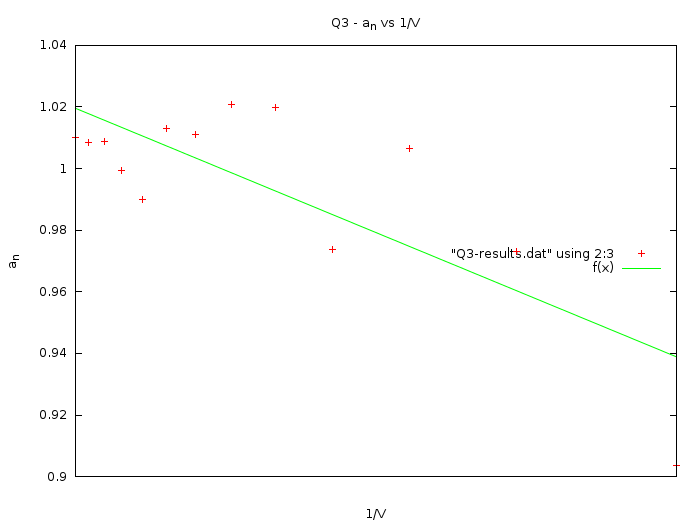
\includegraphics[width=\textwidth]{4-Results/Q3-Verification.png}
    \caption{Q3 $a_n = 0.996294 \pm 0.01123$}
\end{subfigure}

\begin{subfigure}[b]{0.45\textwidth}
   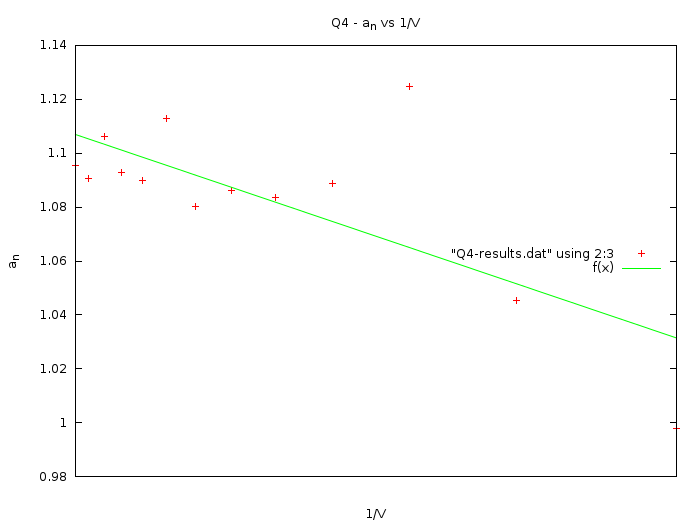
\includegraphics[width=\textwidth]{4-Results/Q4-Verification.png}
    \caption{Q4 $a_n = 1.11538 \pm 0.02026$}
\end{subfigure}

\begin{subfigure}[b]{0.45\textwidth}
    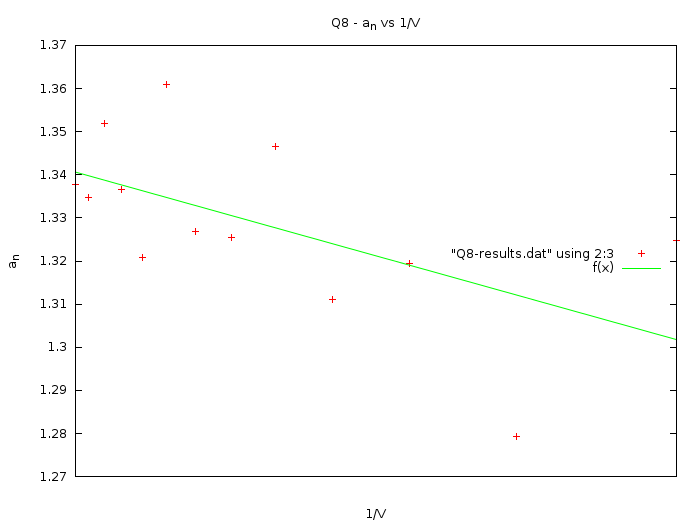
\includegraphics[width=\textwidth]{4-Results/Q8-Verification.png}
    \caption{Q8 $a_n = 1.34759 \pm 0.008933$}
\end{subfigure}
\begin{subfigure}[b]{0.45\textwidth}
    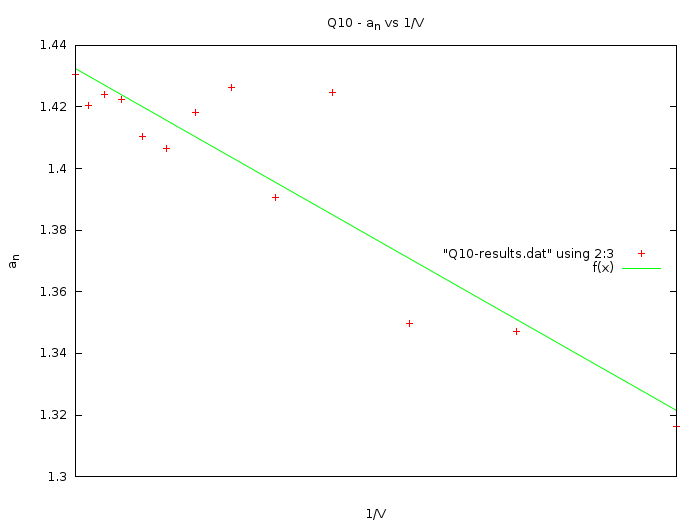
\includegraphics[width=\textwidth]{4-Results/Q10-Verification.png}
    \caption{Q10 $a_n = 1.43679 \pm 0.0152$}
\end{subfigure}
\end{figure}

The above graphs show that in the thermodynamic limit, the calculated values of $a_n$ agree with the $\beta_c$ which is a form of verification to the results from the Wang Landau.

\subsection{Calculating the Partition Function}
The next stage of the project, which is required to calculate the Partition Function, $Z$, is to generate values of $a_n$ at regular intervals between the minimum and maximum energies.
The regular intervals are determined by the energy band width. That means that the midpoints of these intervals for a small grid size for $Q=2$ would be as shown below.
\begin{table}[h]
\centering
\begin{tabular}{|c|c|c|}
\hline
Minimum & Maximum & Midpoint \\ \hline
-2      & -1.9375 & -1.96875 \\ \hline
-1.9375 & -1.875  & -1.90625 \\ \hline
-1.875  & -1.8125 & -1.84375 \\ \hline
...     & ...     & ...      \\ \hline
-0.1875 & -0.125  & -0.15625 \\ \hline
-0.125  & -0.0625 & -0.09375 \\ \hline
-0.0625 & 0.000   & -0.03125 \\ \hline
\end{tabular}
\end{table}

Running the Wang Landau mode of the program with the midpoint as the target energy and the target width as the grid size.

The output from the program for each midpoint when plotted against the energy leads to the plot below.
\begin{figure}[H]
\centering
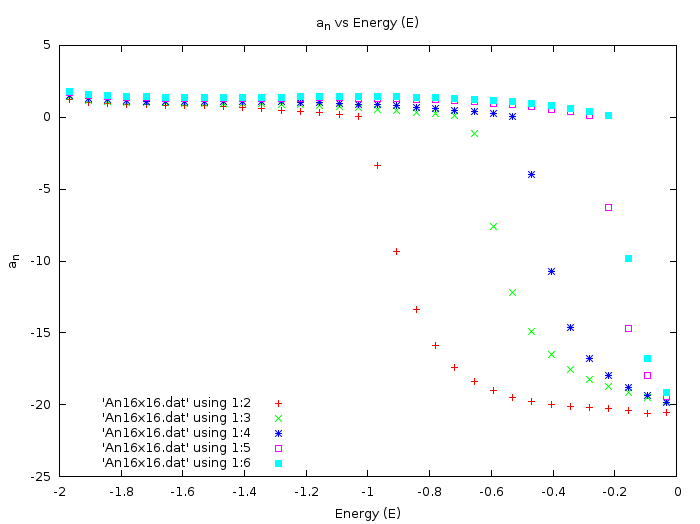
\includegraphics[width=0.75\textwidth]{4-Results/a_n.png}
\caption{Graph showing the plot of $a_n$ across the energy bands for various Q}
\end{figure}

This graph has issues with scaling due to the fact that the maximum energy is dependant on Q.
The maximum energy is dependant on Q because the number of configurations that can represent each energy increases with Q.
A rescaled graph shows a clearer picture for the different Q.

\begin{figure}[H]
\centering
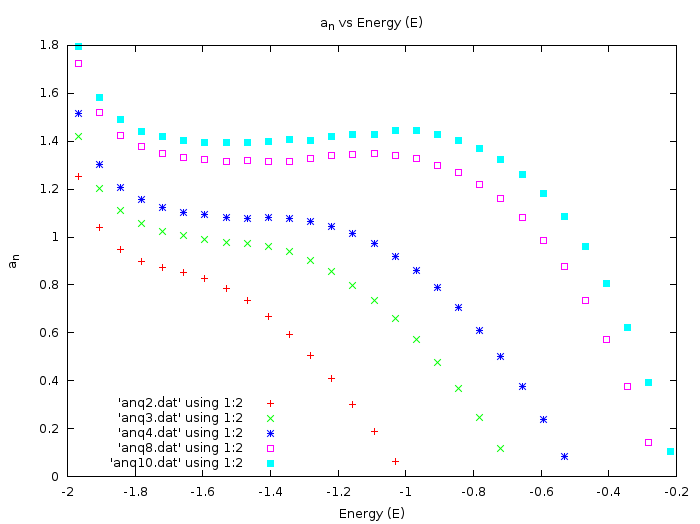
\includegraphics[width=0.75\textwidth]{4-Results/a_n-rescaled.png}
\caption{Graph showing the rescaled plot of $a_n$ across the energy bands for various Q}
\end{figure}

A comparing my results with a similar result from the paper by Guagnelli for Q=10 is shown below.

\begin{figure}[H]
\centering
\begin{subfigure}[b]{0.45\textwidth}
    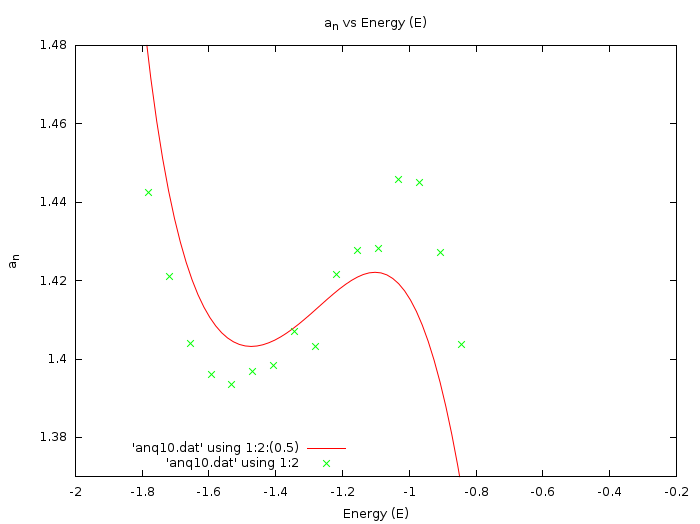
\includegraphics[width=\textwidth]{4-Results/Q10-MyData.png}
    \caption{Q10 Graph showing the rescaled plot of $a_n$ across the energy bands from the program}
\end{subfigure}
\begin{subfigure}[b]{0.45\textwidth}
    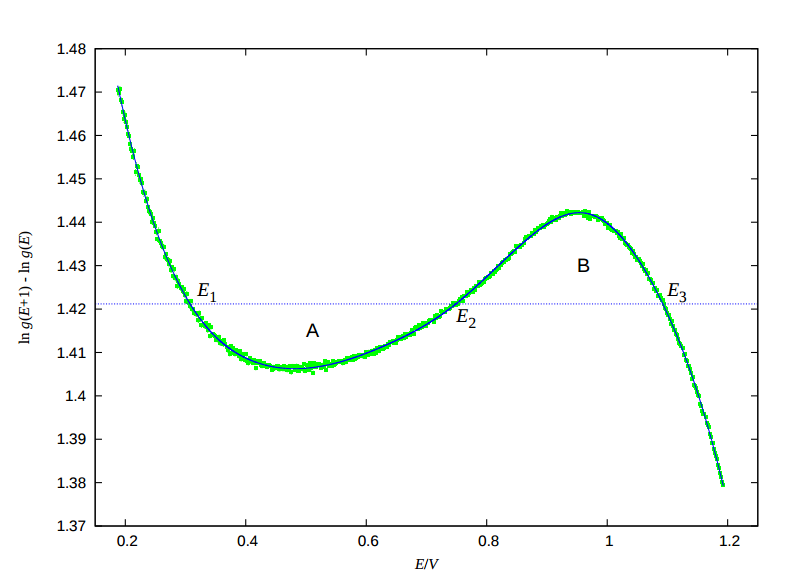
\includegraphics[width=\textwidth]{4-Results/Q10-ComparisonGuagnelli.png}
    \caption{Q10 Graph showing the rescaled plot of $a_n$ across the energy bands from the Guagnelli paper\cite{Montroll1963}}
\end{subfigure}
\end{figure}

The primary discrepancies between the two results is likely to occur due to the difference in lattice sizes used to generate the results and some arbitrary scaling factors used in the simulation.
To calculate the partition function, $Z$, from this data I turned to the symbolic computational mathematics tool kit Mathematica to calculate the constants that keep the Piecewise function of $\log{\rho(E)}$ continuous.
The table \ref{subsec:ContinuityConstants} contains these constants for each of the 5 Q tested, the Null values occur due to the aforementioned scaling issues.

By plotting a Piecewise function in side Mathematica where each component is of the form.
\begin{equation}
f(E) = C_i + a_i(E - E_i)
\end{equation}
$E_i$ is the Midpoint of the interval, $C_i$ is the constant value for that interval to ensure continuity and $a_i$ is the measured value of $a_n$ at the midpoint.
A sample of the piecewise function that Mathematica generates for Q2 is provided in the table at  \ref{subsec:Q2Piecewise}.
Plotting the these Piecewise functions is a good way to ascertain the continuity of the newly generated functions. However due to the way Mathematica renders these functions there appears to be gaps in the rendered output. Included below is the plot for the Q2 piecewise function of $\log{g\left(E\right)}$.
\begin{figure}[H]
\centering
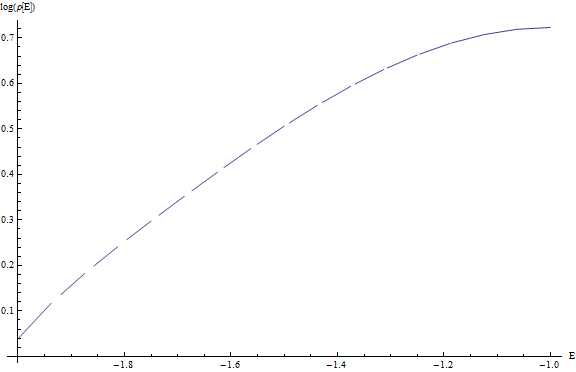
\includegraphics[width=0.75\textwidth]{4-Results/Q2Log(g(E)).png}
\caption{Graph showing the $\log{g\left(E\right)}$ vs E}
\end{figure}
The plots for Q3, Q4, Q8, Q10 can be found in the appendix at \ref{subsec:QLogg}. All the plots show similar behaviour for all the various values of Q.
Now the only piece of information that remains to provide the complete Density of States is the constant, $c_0$ that is added to all of the piecewise functions.
As explained earlier this value is calculated using the following equation
\begin{equation}
C_0 = \frac{2L^2}{\int g(E) dE}
\end{equation}
In this case, $g(E)$ is the incomplete Density of States. 
The integral can be computed easily using the tools provided by Mathematica however it could also be computed using a simple Simpson's rule integrator due to the linear nature of the approximations used to calculate the Density of States.
After adding this constant to the incomplete Density of States, you get the complete Density of States for that simulation.
The next stage of the processing for the Mathematica program is to calculate the Partition Function.
The partition function can be written in the form.
\begin{equation}
\mathcal{Z} = \int g(E) e^{-\beta E} dE
\end{equation}
Using Mathematica to perform the integration numerically across the sampled energy range you can extract the Partition Function as a function of $\beta$.
With this done the analysis of this part of the project is complete.
\section{Wang Landau with a Twist}
After modifying the configuration file to add the twist into the simulation and running the simulation across various lattice sizes.
After extracting the data from the programs output files and importing it into Mathematica the code is nearly indistinguishable from that described earlier for the Wang Landau data so to ensure that I am not repeating any material I will describe the next stages of analysis here. The plots of the incomplete Density of States are available in the appendix at \ref{subsec:QLoggInt}.

Having now calculated the Partition Functions for the untwisted $Z$ and twisted $Z^*$ lattice, the next stage is to calculate the interface free energy. The Interface Free Energy as described earlier can be written as 
\begin{equation}
F_{I}\left(L\right)=-\log{\frac{Z^*}{Z}} - \log{L}
\end{equation}
The Mathematica notebook provided in the appendix \ref{subsec:MathematicaNotebook} is a copy of the working code used to perform all of the analysis for the Wang Landau model.
Taking the results from the Mathematica notebook for the Interface Free Energy at $\beta_c$ and using the form for the interface tension \cite{1111.4832}.
\begin{equation}
\sigma = \lim_{L\to\infty} \frac{F_{I}}{V_{D-1}}
\end{equation}

Taking the results from the Mathematica notebook for the various grid sizes and taking a fit of the plot to the thermodynamic limit leads to the results below for the interface tension $\sigma$ at $\beta_c$.
\begin{figure}[H]
\centering
\begin{subfigure}[b]{0.45\textwidth}
    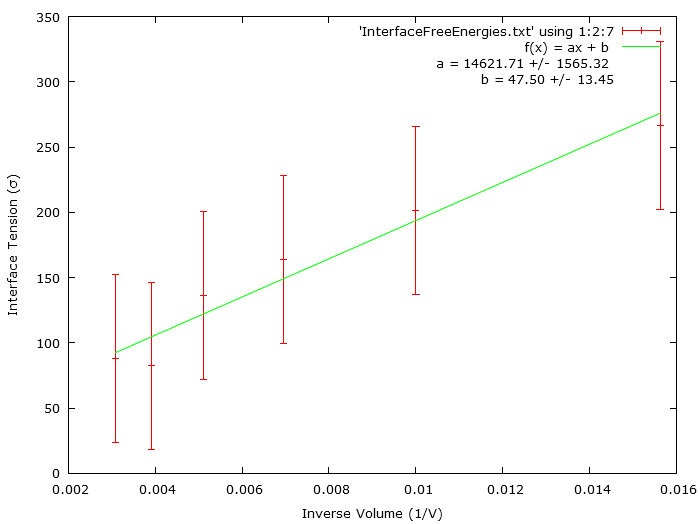
\includegraphics[width=\textwidth]{4-Results/Q2-InterfaceTension.png}
    \caption{Q2 $\sigma = -0.01404 \pm 0.00236$}
\end{subfigure}
\begin{subfigure}[b]{0.45\textwidth}
    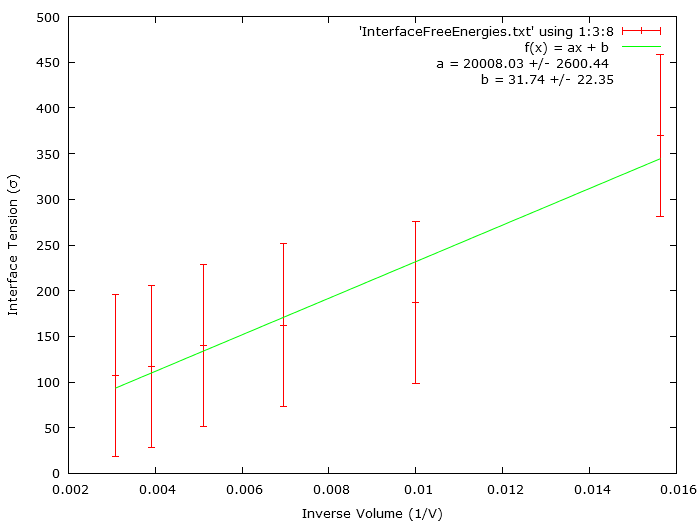
\includegraphics[width=\textwidth]{4-Results/Q3-InterfaceTension.png}
    \caption{Q3 $\sigma = -0.02238 \pm 0.00815$}
\end{subfigure}

\begin{subfigure}[b]{0.45\textwidth}
   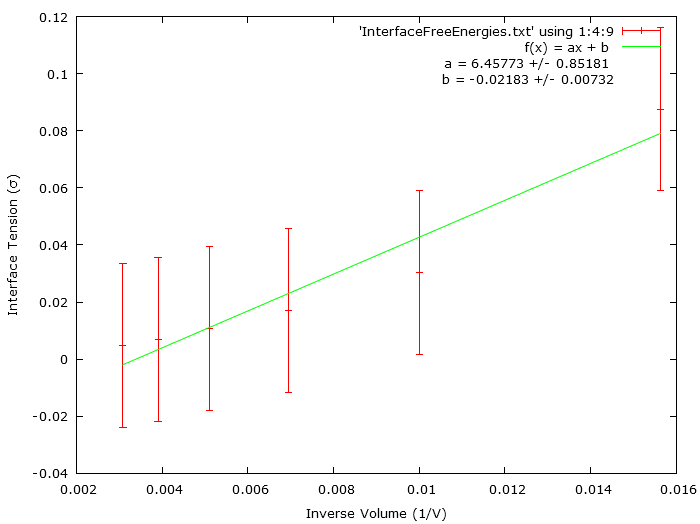
\includegraphics[width=\textwidth]{4-Results/Q4-InterfaceTension.png}
    \caption{Q4 $\sigma = -0.02183 \pm 0.00732$}
\end{subfigure}

\begin{subfigure}[b]{0.45\textwidth}
    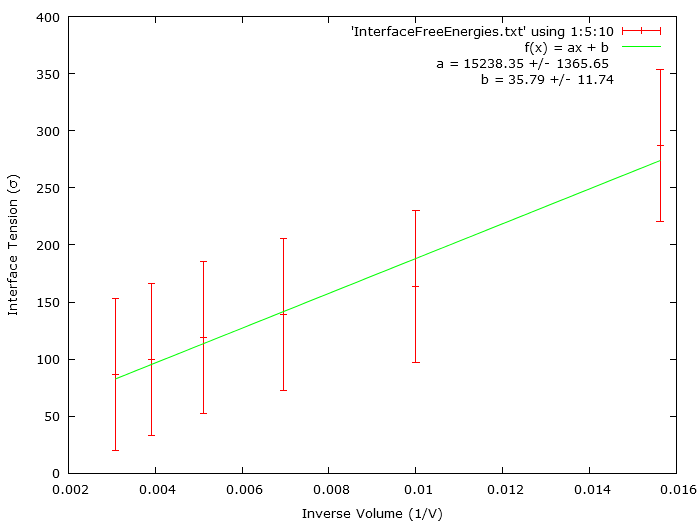
\includegraphics[width=\textwidth]{4-Results/Q8-InterfaceTension.png}
    \caption{Q8 $\sigma = -0.01650 \pm 0.00534$}
\end{subfigure}
\begin{subfigure}[b]{0.45\textwidth}
    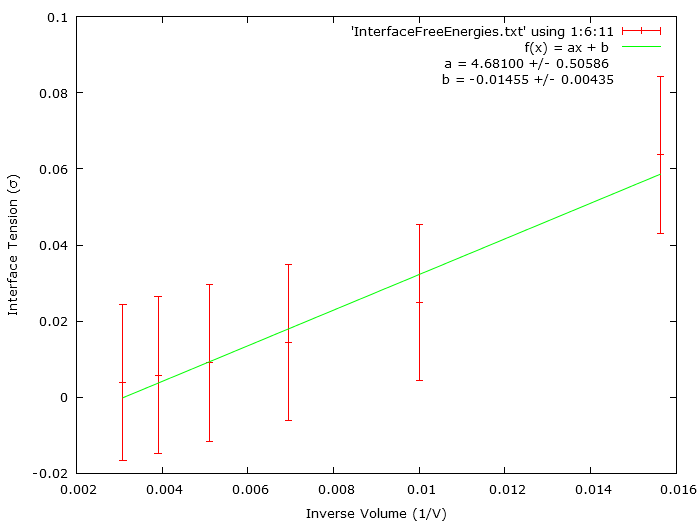
\includegraphics[width=\textwidth]{4-Results/Q10-InterfaceTension.png}
    \caption{Q10 $\sigma = =0.01455 \pm 0.00435$}
\end{subfigure}
\end{figure}
This information isn't useful for determining the behaviour of the Interface tension reformatting the output from the Mathematica notebook to extract the interface tension at a range of $\beta$ and for all of the lattice sizes provides further insight into the behaviour of the interface tension.

\begin{figure}[H]
\centering
\begin{subfigure}[b]{0.45\textwidth}
    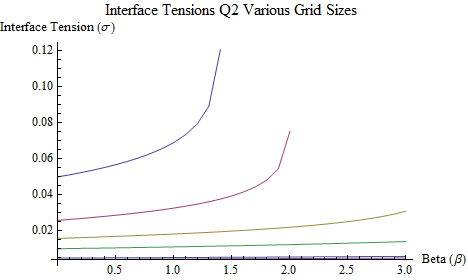
\includegraphics[width=\textwidth]{4-Results/Q2VariousGridSizesTensions.png}

\end{subfigure}
\begin{subfigure}[b]{0.45\textwidth}
    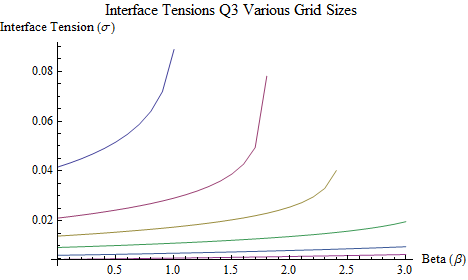
\includegraphics[width=\textwidth]{4-Results/Q3VariousGridSizesTensions.png}

\end{subfigure}

\begin{subfigure}[b]{0.45\textwidth}
   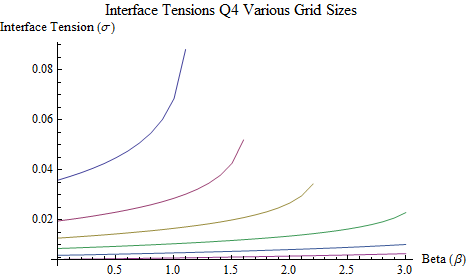
\includegraphics[width=\textwidth]{4-Results/Q4VariousGridSizesTensions.png}

\end{subfigure}

\begin{subfigure}[b]{0.45\textwidth}
    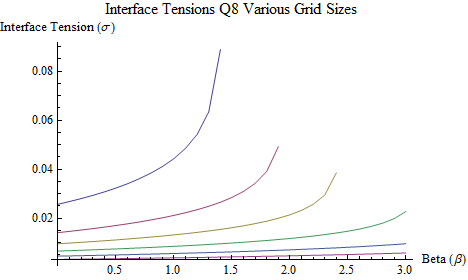
\includegraphics[width=\textwidth]{4-Results/Q8VariousGridSizesTensions.png}

\end{subfigure}
\begin{subfigure}[b]{0.45\textwidth}
    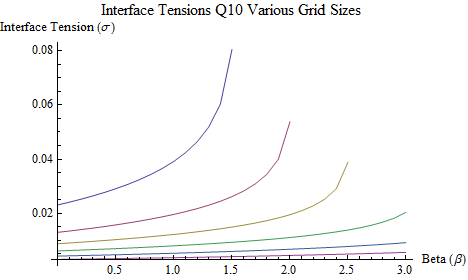
\includegraphics[width=\textwidth]{4-Results/Q10VariousGridSizesTensions.png}

\end{subfigure}
\end{figure}

In the graphs above you can clearly see that the interface tension on the smaller grids rapidly increases with $\beta$. This is primarily due to the fact that on a smaller lattice, the affect of the twist is significantly larger than on a bigger lattice.
On the larger lattices which almost appear to be linear in this scale you would expect to have the same or similar behaviour over a larger $\beta$ range.
For a large $\beta$, low T, the twist artificially creates an interface that leads to an increase in the energy. The overall effect of the interface to the systems energy is directly proportional to the lattice size which would explain why for the larger lattice sizes the tension doesn't grow rapidly in the range of $\beta$ sampled.